\documentclass[crop,border={2pt 2pt 2pt 2pt},tikz]{standalone}
\usepackage{braket}
\usepackage{bbold}
\usepackage{bm}
\usepackage{amsmath}

\usetikzlibrary{backgrounds,decorations.markings, calc}
\tikzset{>=latex}
\tikzset{->-/.style={decoration={
  markings,
  mark=at position .55 with {\arrow{>}}},postaction={decorate}}}
\begin{document}
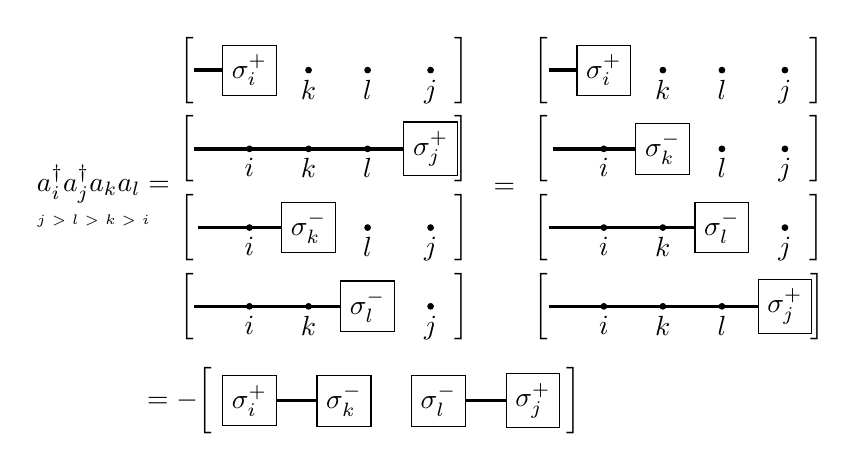
\begin{tikzpicture}[scale = 1]

    \coordinate[draw] (i) at (0,0);
    \coordinate[draw] (j) at (2.3,0);
    \coordinate[draw] (k) at (0.75,0);
    \coordinate[draw] (l) at (1.5,0);
    
    \node[text width = 2cm] at ($(i) + (-1.7, -1.6)$) {$a^\dagger_i a^\dagger_j a_k a_l = $ \\ {\tiny $j>l>k>i$}};
    \node[] at ($(i) + (-0.8, 0)$) {$\bigg[$};
    \draw[black,very thick] ($(i) + (-0.7,0)$) -- (i) node[draw,thin, fill = white,  anchor = center] {$\sigma^{+}_i$};

    \draw[fill, black] (j) circle (1pt) node[anchor = north] {$j$};
    \draw[fill, black] (k) circle (1pt) node[anchor = north] {$k$};
    \draw[fill, black] (l) circle (1pt) node[anchor = north] {$l$};

    \node[] at ($(j) + (0.4, 0)$) {$\bigg]$};
    
    \begin{scope}[yshift = -1cm ]
        \coordinate[draw] (i) at (0,0);
        \coordinate[draw] (j) at (2.3,0);
        \coordinate[draw] (k) at (0.75,0);
        \coordinate[draw] (l) at (1.5,0);
        
        \node[] at ($(i) + (-0.8, 0)$) {$\bigg[$};

        \draw[black,very thick] ($(j) + (-3,0)$) -- (j) node[draw,thin, fill = white, anchor = center] {$\sigma^{+}_j$};

        \draw[fill, black] (i) circle (1pt) node[anchor = north] {$i$};
        \draw[fill, black] (k) circle (1pt) node[anchor = north] {$k$};
        \draw[fill, black] (l) circle (1pt) node[anchor = north] {$l$};

        \node[] at ($(j) + (0.4, 0)$) {$\bigg] $}; 

        % \node[] at ($(j) + (1.5, 0)$) {$j > i$}; 

    \end{scope}
    


    \begin{scope}[yshift = -2cm ]
        \coordinate[draw] (i) at (0,0);
        \coordinate[draw] (j) at (2.3,0);
        \coordinate[draw] (k) at (0.75,0);
        \coordinate[draw] (l) at (1.5,0);
        
        \node[] at ($(i) + (-0.8, 0)$) {$\bigg[$};

        \draw[black,very thick] ($(k) + (-1.4,0)$) -- (k) node[draw,thin, fill = white, anchor = center] {$\sigma^{-}_k$};

        \draw[fill, black] (i) circle (1pt) node[anchor = north] {$i$};
        \draw[fill, black] (j) circle (1pt) node[anchor = north] {$j$};
        \draw[fill, black] (l) circle (1pt) node[anchor = north] {$l$};

        \node[] at ($(j) + (0.4, 0)$) {$\bigg] $}; 

        % \node[] at ($(j) + (1.5, 0)$) {$j > i$}; 

    \end{scope}

    \begin{scope}[yshift = -3cm ]
        \coordinate[draw] (i) at (0,0);
        \coordinate[draw] (j) at (2.3,0);
        \coordinate[draw] (k) at (0.75,0);
        \coordinate[draw] (l) at (1.5,0);
        
        \node[] at ($(i) + (-0.8, 0)$) {$\bigg[$};

        \draw[black,very thick] ($(l) + (-2.2,0)$) -- (l) node[draw,thin, fill = white, anchor = center] {$\sigma^{-}_l$};

        \draw[fill, black] (i) circle (1pt) node[anchor = north] {$i$};
        \draw[fill, black] (j) circle (1pt) node[anchor = north] {$j$};
        \draw[fill, black] (k) circle (1pt) node[anchor = north] {$k$};

        \node[] at ($(j) + (0.4, 0)$) {$\bigg] $}; 

        % \node[] at ($(j) + (1.5, 0)$) {$j > i$}; 

    \end{scope}
    

    \begin{scope}[xshift = 4.5cm ]
        \coordinate[draw] (i) at (0,0);
        \coordinate[draw] (j) at (2.3,0);
        \coordinate[draw] (k) at (0.75,0);
        \coordinate[draw] (l) at (1.5,0);
        
        \node[text width = 2cm] at ($(i) + (-0.4, -1.5)$) {$=$};
        \node[] at ($(i) + (-0.8, 0)$) {$\bigg[$};
        \draw[black,very thick] ($(i) + (-0.7,0)$) -- (i) node[draw,thin, fill = white,  anchor = center] {$\sigma^{+}_i$};
    
        \draw[fill, black] (j) circle (1pt) node[anchor = north] {$j$};
        \draw[fill, black] (k) circle (1pt) node[anchor = north] {$k$};
        \draw[fill, black] (l) circle (1pt) node[anchor = north] {$l$};
    
        \node[] at ($(j) + (0.4, 0)$) {$\bigg]$};
        
        \begin{scope}[yshift = -3cm ]
            \coordinate[draw] (i) at (0,0);
            \coordinate[draw] (j) at (2.3,0);
            \coordinate[draw] (k) at (0.75,0);
            \coordinate[draw] (l) at (1.5,0);
            
            \node[] at ($(i) + (-0.8, 0)$) {$\bigg[$};
    
            \draw[black,very thick] ($(j) + (-3,0)$) -- (j) node[draw,thin, fill = white, anchor = center] {$\sigma^{+}_j$};
    
            \draw[fill, black] (i) circle (1pt) node[anchor = north] {$i$};
            \draw[fill, black] (k) circle (1pt) node[anchor = north] {$k$};
            \draw[fill, black] (l) circle (1pt) node[anchor = north] {$l$};
    
            \node[] at ($(j) + (0.3, 0)$) {$ \ \ \bigg] $}; 
    
            % \node[] at ($(j) + (1.5, 0)$) {$j > i$}; 
    
        \end{scope}
        
    
    
        \begin{scope}[yshift = -1cm ]
            \coordinate[draw] (i) at (0,0);
            \coordinate[draw] (j) at (2.3,0);
            \coordinate[draw] (k) at (0.75,0);
            \coordinate[draw] (l) at (1.5,0);
            
            \node[] at ($(i) + (-0.8, 0)$) {$\bigg[$};
    
            \draw[black,very thick] ($(k) + (-1.4,0)$) -- (k) node[draw,thin, fill = white, anchor = center] {$\sigma^{-}_k$};
    
            \draw[fill, black] (i) circle (1pt) node[anchor = north] {$i$};
            \draw[fill, black] (j) circle (1pt) node[anchor = north] {$j$};
            \draw[fill, black] (l) circle (1pt) node[anchor = north] {$l$};
    
            \node[] at ($(j) + (0.4, 0)$) {$\bigg] $}; 
    
            % \node[] at ($(j) + (1.5, 0)$) {$j > i$}; 
    
        \end{scope}
    
        \begin{scope}[yshift = -2cm ]
            \coordinate[draw] (i) at (0,0);
            \coordinate[draw] (j) at (2.3,0);
            \coordinate[draw] (k) at (0.75,0);
            \coordinate[draw] (l) at (1.5,0);
            
            \node[] at ($(i) + (-0.8, 0)$) {$\bigg[$};
    
            \draw[black,very thick] ($(l) + (-2.2,0)$) -- (l) node[draw,thin, fill = white, anchor = center] {$\sigma^{-}_l$};
    
            \draw[fill, black] (i) circle (1pt) node[anchor = north] {$i$};
            \draw[fill, black] (j) circle (1pt) node[anchor = north] {$j$};
            \draw[fill, black] (k) circle (1pt) node[anchor = north] {$k$};
    
            \node[] at ($(j) + (0.4, 0)$) {$\bigg] $}; 
    
            % \node[] at ($(j) + (1.5, 0)$) {$j > i$}; 
    
        \end{scope}
        
    
    \end{scope}


    \begin{scope}[yshift = -4.2cm ]
        \coordinate[draw] (i) at (0,0);
        \coordinate[draw] (j) at (3.6,0);
        \coordinate[draw] (k) at (1.2,0);
        \coordinate[draw] (l) at (2.4,0);
        
        \node[text width = 2cm] at ($(i) + (-0.3, 0)$) {$= - \bigg[$};
        % \node[] at ($(i) + (-0.8, 0)$) {$ - \bigg[$};


        
        \draw[black,very thick] (l) -- (j) node[draw,thin, fill = white,  anchor = center, pos = 1] {$\sigma^{+}_j$} node[draw,thin, fill = white,  anchor = center, pos = 0] {$\sigma^{-}_l$};
        
        
        % \draw[black,very thick] (k) -- (l) node[draw,thin, fill = white,  anchor = center, pos = 1] {$\sigma^{-}_l$} node[draw,thin, fill = white,  anchor = center, pos = 0] {$\sigma^{+}_j$};

        \draw[black,very thick] (i) -- (k) node[draw,thin, fill = white,  anchor = center, pos = 0] {$\sigma^{+}_i $} node[draw,thin, fill = white,  anchor = center, pos = 1] {$\sigma^{-}_k$};


        % \draw[black,very thick] (i) -- (k) node[draw,thin, fill = white,  anchor = center, pos = 0] {$\sigma^{+}_i \sigma^{z}_i$} node[draw,thin, fill = white,  anchor = center, pos = 1] {$\sigma^{-}_k \sigma^{z}_k$};

        % \draw[black,very thick] ($(j) + (-0.7,0)$) -- (i) node[draw,thin, fill = white,  anchor = center] {$\sigma^{+}_i$};
        % \draw[black,very thick] ($(k) + (-0.7,0)$) -- (i) node[draw,thin, fill = white,  anchor = center] {$\sigma^{+}_i$};
        % \draw[black,very thick] ($(l) + (-0.7,0)$) -- (i) node[draw,thin, fill = white,  anchor = center] {$\sigma^{+}_i$};

    
        \node[] at ($(j) + (0.4, 0)$) {$ \ \ \bigg]$};
        
    
    \end{scope}


\end{tikzpicture}
\end{document}